\levelstaynon{Ch. 8 (AO)}
\leveldownnon{Problem 8.4.1}
\textbf{(a):} Verify that Eq. (8.2) is the solution to the diffusion equation with perfectly reflecting barriers at $x=\pm a$.

Suppose there exists a separable solution of the form $p(x,t) = f(x) g(t)$. This implies that
\begin{equation}
f(x) g'(t) = D f''(x) g(t)
\end{equation}
by plugging $p(x, t)$ in the diffusion equation. From here it follows that
\begin{equation}
\frac{f''(x)}{f(x)} = \frac{1}{D} \frac{g'(t)}{g(t)}.
\end{equation}
As each side of this equation is a function of a different independent variable, the only way this can happen is if 
\begin{equation}
\frac{f''(x)}{f(x)} = \frac{1}{D} \frac{g'(t)}{g(t)} = -\lambda,~\text{where}~\lambda=\text{constant}.
\end{equation}
The solution to the L.H.S of this equation is given by
\begin{equation}
f(x) = a \times \cos(\sqrt{\lambda} x) + b \times \sin(\sqrt{\lambda} x).
\end{equation}
By symmetry, we assume $b=0$. The solution to the R.H.S of this equation is given by
\begin{equation}
g(t) = c \times \exp(- D \lambda t).
\end{equation}
The reflecting boundaries imply that $\partial p(x,t)/\partial x |_{x=\pm a} = 0$.  This happens when
\begin{equation}
\sqrt{\lambda} = \frac{n \pi}{a}~~\text{where}~n \in \{0, 1, 2, \ldots\}.
\end{equation}
In other words, the general solution to this equation is of the form
\begin{equation}
p(x,t) = \sum_{n=0}^{\infty} c_n \cos\bigg(\frac{n \pi}{a} x \bigg) \exp\bigg(-\frac{n^2 \pi^2}{a^2} D t \bigg). \label{eq:gen_soln_refl_bound}
\end{equation}
To determine the values of $c_n$, we use the initial condition $p(x, t=0) = \delta(x)$. It is helpful to note that
\begin{equation}
\delta(\xi) = \sum_{n=-\infty}^{\infty} e^{2 \pi n i \xi}. \nonumber
\end{equation}
From here it follows that
\begin{eqnarray}
\delta(x/2a) &=& \sum_{n=-\infty}^{\infty} e^{i n \pi x /a} \nonumber \\
&=& 1 + 2 \sum_{n=1}^{\infty} \cos\bigg(\frac{n \pi}{a} x \bigg).
\end{eqnarray}
As $\delta(c x) = \delta(x) / |c|$, one has that
\begin{equation}
\delta(x/2a) = \delta(x) \times 2 |a| = 1 + 2 \sum_{n=1}^{\infty} \cos\bigg(\frac{n \pi}{a} x \bigg), \nonumber
\end{equation}
in other words\footnote{We drop the $|a|$ as $a>0$.}
\begin{equation}
\delta(x) = \frac{1}{2a} + \frac{1}{a} \sum_{n=1}^{\infty} \cos\bigg(\frac{n \pi}{a} x \bigg).
\end{equation}
Matching each term in this sum with terms from Eq. (\ref{eq:gen_soln_refl_bound}) [evaluated at $t=0$] gives us $c_0 = 1/2a$ and $c_i = 1/a$ for all $i\geq 1$. From here it follows that
\begin{equation}
\boxed{p(x,t) = \frac{1}{2 a} +  \frac{1}{a}\sum_{n=1}^{\infty} \cos\bigg(\frac{n \pi}{a} x \bigg) \exp\bigg(-\frac{n^2 \pi^2}{a^2} D t \bigg)}~.
\end{equation}
This matches Eq. (8.2) from the textbook.

\textbf{(b):} Verify that Eq. (8.6) is the solution to the diffusion equation with perfectly absorbing barriers at $x=\pm a$.

Assume a separable solution of the form $p(x,t) = h(x) k(t)$.
In an analogous manner to part (a), the solution for $h(x)$ is given by
\begin{equation}
h(x) = a \times \cos(\sqrt{\lambda} x) + b \times \sin(\sqrt{\lambda} x).
\end{equation}
By symmetry, we assume $b=0$. The solution for $k(t)$ is given by
\begin{equation}
k(t) = c \times \exp(- D \lambda t).
\end{equation}
From the absorbing boundary conditions $p(x=\pm a, t) = 0$, one has that
\begin{equation}
\sqrt{\lambda} = \frac{(2n+1) \pi}{2a} ~~\text{where}~n \in \{0, 1, 2, \ldots\}.
\end{equation}
The general solution to this equation is of the form
\begin{eqnarray}
p(x,t) &=& \sum_{n=0}^{\infty} c_n \cos\bigg(\bigg[\frac{(2n+1) \pi}{2a} \bigg]  x \bigg) \exp\bigg(-\bigg[\frac{(2n+1) \pi}{2a} \bigg]^2 D t \bigg) \nonumber \\
&=& \sum_{n=-\infty}^{\infty} c_n' \exp\bigg(i\bigg[\frac{(2n+1) \pi}{2a} \bigg]  x \bigg) \exp\bigg(-\bigg[\frac{(2n+1) \pi}{2a} \bigg]^2 D t \bigg) \nonumber \\
&=& \exp\bigg(i\frac{\pi x}{2a} \bigg) \sum_{n=-\infty}^{\infty} c_n' \exp\bigg(i\frac{n \pi}{a} x \bigg) \exp\bigg(-\bigg[\frac{(2n+1) \pi}{2a} \bigg]^2 D t \bigg). \label{eq:gen_soln_abs_bound}
\end{eqnarray}
Using the initial condition $p(x, t=0) = \delta(x)$  and that\footnote{We also use the fact that $f(x)\delta(x)=f(0)\delta(x)$ and that $\exp(i\pi x/2a)|_{x=0} = 1$.}
\begin{equation}
\frac{\delta(x/2a)}{2 a} = \delta(x)= \frac{1}{2 a }\sum_{n=-\infty}^{\infty} e^{i n \pi x /a},
\end{equation}
one has that $c_n' = 1/ 2a$ for all $n$. From here it follows that
\begin{eqnarray}
p(x,t) &=& \frac{1}{2a} \exp\bigg(i\frac{\pi x}{2a} \bigg) \sum_{n=-\infty}^{\infty} \exp\bigg(i\frac{n \pi}{a} x \bigg) \exp\bigg(-\bigg[\frac{(2n+1) \pi}{2a} \bigg]^2 D t \bigg) \nonumber \\
&=& \frac{1}{2a} \sum_{n=-\infty}^{\infty} \exp\bigg(i\bigg[\frac{(2n+1) \pi}{2a} \bigg] x \bigg) \exp\bigg(-\bigg[\frac{(2n+1) \pi}{2a} \bigg]^2 D t \bigg) \nonumber \\
&=& \boxed{\frac{1}{a} \sum_{n=0}^{\infty} \cos\bigg(\bigg[\frac{(2n+1) \pi}{2a} \bigg] x \bigg) \exp\bigg(-\bigg[\frac{(2n+1) \pi}{2a} \bigg]^2 D t \bigg)}~.
\end{eqnarray}
This matches Eq. (8.6) from the textbook.

\levelstaynon{Problem 8.4.2}
When one of the reflecting (or absorbing) boundaries is absent, the solution to the diffusion equation via the method of images can be written down in closed form as
\begin{equation}
p(x,t) = \frac{1}{\sqrt{4 \pi D t} } \bigg\{ \exp \bigg( - \frac{(x-x_0)^2}{4Dt}\bigg) \pm \exp \bigg( - \frac{(x-[2a-x_0])^2}{4Dt}\bigg) \bigg\}, \label{eq:diff_on_semi_infinite_line}
\end{equation}
where the $+$ ($-$) sign corresponds to a reflecting (absorbing) boundary at $x=+a$. Of course, $(2a-x_0)$ is the location of the image particle with respect the lone boundary at $x=+a$ when $t=0$. See Fig. (\ref{fig:8p2}) for plots $p(x,t)$ versus time.

\begin{figure}[hb!]
\centering
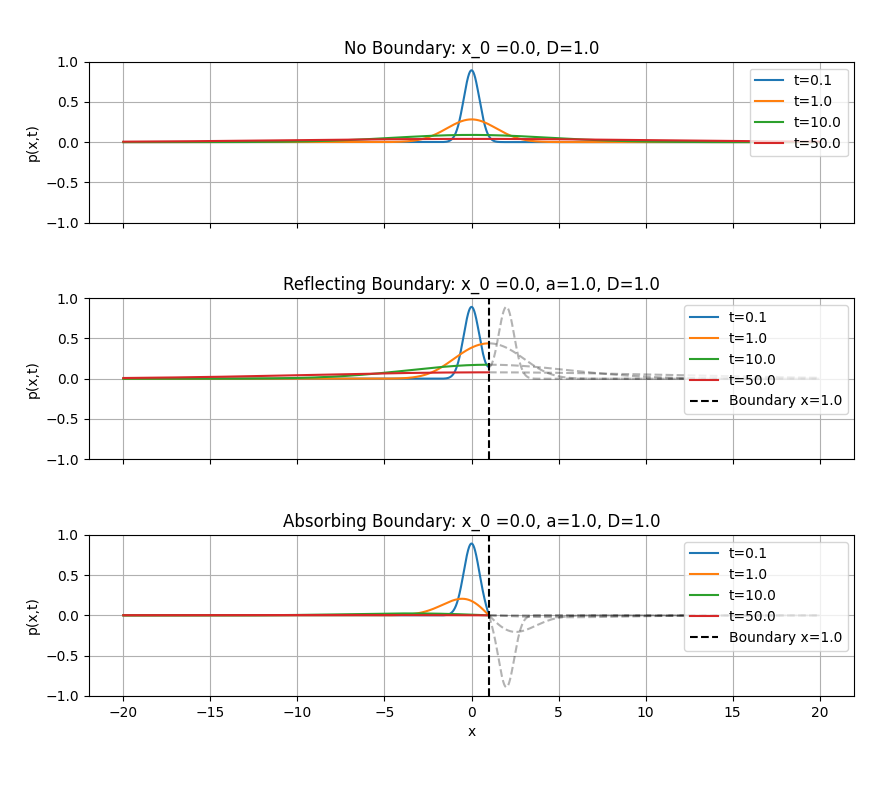
\includegraphics[width=14cm]{reflecting_absorbing_dynamics.png}
    \caption{Dynamics of Eq. (\ref{eq:diff_on_semi_infinite_line}) for a reflecting (middle plot) and absorbing (bottom plot) boundary at $x=1$. The top plot shows the dynamics when there is no boundary.}
    \label{fig:8p2}
\end{figure}

\levelstaynon{Problem 8.4.3}
\textbf{(a):} Show that Eq. (8.2) and Eq. (8.10) are identical using Poisson's summation formula.

Eq. (8.10) is given by
\begin{equation}
p(x,t) = \frac{1}{\sqrt{4 \pi D t}} \sum_{n=-\infty}^{\infty} \exp \bigg( -\frac{(x+2na)^2}{4Dt} \bigg). \nonumber
\end{equation}
Defining
\begin{equation}
f(q) = \frac{1}{\sqrt{4 \pi D t}} \exp \bigg( -\bigg[q + \frac{x}{\sqrt{4Dt}}\bigg]^2 \bigg) \nonumber
\end{equation}
and 
\begin{equation}
\lambda = a/\sqrt{Dt} \nonumber
\end{equation} 
means that
\begin{equation}
p(x,t)=\sum_{n=-\infty}^{\infty} f(\lambda n). \nonumber
\end{equation}
The Fourier transform of $f(q)$ is given by
\begin{eqnarray}
\tilde{f}(k) &=& \int_{-\infty}^{\infty} dq~e^{-i k q}~f(q) \nonumber \\
&=& \frac{1}{\sqrt{4 \pi D t}} \int_{-\infty}^{\infty} dq~\exp\bigg\{-\bigg[q^2 + 2q\bigg(\frac{x}{\sqrt{4Dt}} + \frac{ik}{2}\bigg)\bigg]-\frac{x^2}{4Dt}\bigg\}. \nonumber
\end{eqnarray}
It is helpful to note that
\begin{equation}
-\bigg[q^2 + 2q\bigg(\frac{x}{\sqrt{4Dt}} + \frac{ik}{2}\bigg)\bigg] = -\bigg[q+\bigg(\frac{x}{\sqrt{4Dt}} + \frac{ik}{2}\bigg) \bigg]^2 + \frac{x^2}{4Dt}+ \frac{i k x}{\sqrt{4Dt}} - \frac{k^2}{4}.
\end{equation}
From here it follows that
\begin{eqnarray}
\tilde{f}(k)&=& \frac{1}{\sqrt{4 \pi D t}} \int_{-\infty}^{\infty} dq~\exp\bigg\{-\bigg[q^2 + 2q\bigg(\frac{x}{\sqrt{4Dt}} + \frac{ik}{2}\bigg)\bigg]-\frac{x^2}{4Dt}\bigg\} \nonumber \\
&=& \frac{1}{\sqrt{4 \pi D t}} \exp\bigg(-\cancel{\frac{x^2}{4Dt}} + \cancel{\frac{x^2}{4Dt}} + \frac{ikx}{\sqrt{4Dt}} - \frac{k^2}{4}\bigg) \underbrace{\int_{-\infty}^{\infty} dq~\exp\bigg(-\bigg[q + \bigg(\frac{x}{\sqrt{4Dt}} + \frac{ik}{2}\bigg)\bigg]^2\bigg)}_{\sqrt{\pi}} \nonumber \\
&=& \frac{1}{\sqrt{4 D t}} \exp\bigg(\frac{ikx}{\sqrt{4Dt}} - \frac{k^2}{4}\bigg).
\end{eqnarray}
When $k=2\pi n/\lambda$ with $\lambda = a/\sqrt{Dt}$, one has that
\begin{eqnarray}
\frac{1}{\lambda} \sum_{n=-\infty}^{\infty} \tilde{f}\bigg(\frac{2 \pi n}{\lambda}\bigg) &=& \frac{\sqrt{Dt}}{a} \bigg\{ \sum_{n=-\infty}^{\infty} \frac{1}{\sqrt{4 D t}} \times \exp \bigg( - \frac{1}{4} \frac{4 \pi^2 n^2 D t}{a^2} + \frac{i 2 \pi n \sqrt{Dt} x}{a \sqrt{4Dt}} \bigg) \bigg\} \nonumber \\
&=&  \frac{1}{2a} \sum_{n=-\infty}^{\infty} \exp \bigg( - \frac{ \pi^2 n^2 Dt}{a^2} + \frac{i \pi nx}{a} \bigg) \nonumber \\
&=&  \frac{1}{2a} \sum_{n=-\infty}^{\infty} \exp\bigg(\frac{i \pi nx}{a} \bigg) \exp \bigg( - \frac{ \pi^2 D t n^2}{a^2}\bigg)  \nonumber \\
&=&  \frac{1}{2a} + \frac{1}{a} \sum_{n=1}^{\infty} \cos\bigg( \frac{ \pi nx}{a} \bigg) \exp \bigg( - \frac{ \pi^2 D t n^2}{a^2}\bigg) \nonumber
\end{eqnarray}
which matches Eq. (8.10) from the text book. Therefore, by Poisson's summation formula, one has that
\begin{eqnarray}
p(x,t) &=& \boxed{\frac{1}{\sqrt{4 \pi D t}} \sum_{n=-\infty}^{\infty} \exp \bigg( -\frac{(x+2na)^2}{4Dt} \bigg)} ~~\text{[Eq. (8.2) from textbook]}  \nonumber  \\
&=& \sum_{n=-\infty}^{\infty} f(\lambda n)~~(\text{with}~\lambda = a/\sqrt{Dt}) \nonumber \\ 
&=& \frac{1}{\lambda} \sum_{n=-\infty}^{\infty} \tilde{f}\bigg(\frac{2 \pi n}{\lambda}\bigg) \nonumber \\
&=& \boxed{\frac{1}{2a} + \frac{1}{a} \sum_{n=1}^{\infty} \cos\bigg( \frac{ \pi nx}{a} \bigg) \exp \bigg( - \frac{ \pi^2 D t n^2}{a^2}\bigg)}~~\text{[Eq. (8.10) from textbook]}. \nonumber 
\end{eqnarray}




\textbf{(b):} Show that Eq. (8.6) and Eq. (8.12) are identical using Poisson's summation formula.

Eq. (8.12) is given by
\begin{equation}
p(x,t) = \frac{1}{\sqrt{4 \pi D t}} \sum_{n=-\infty}^{\infty} (-1)^n \exp \bigg( -\frac{(x+2na)^2}{4Dt} \bigg). \nonumber 
\end{equation}
Note that $(-1)^n = e^{i\pi n}$ for all $n\in \mathbb{Z}$, allowing us to rewrite this expression as
\begin{equation}
p(x,t) = \frac{1}{\sqrt{4 \pi D t}} \sum_{n=-\infty}^{\infty} \exp \bigg(i\pi n -\frac{(x+2na)^2}{4Dt} \bigg). \nonumber 
\end{equation}
From here we identify $f(q)$ as
\begin{equation}
f(q) = \frac{1}{\sqrt{4 \pi D t} } \exp\bigg( i\pi \frac{q}{\lambda} - \bigg[q + \frac{x}{\sqrt{4Dt}}\bigg]^2\bigg) \nonumber
\end{equation}
where $\lambda=a/\sqrt{Dt}$. We note that
\begin{equation}
p(x,t)=\sum_{n=-\infty}^{\infty} f(\lambda n). \nonumber
\end{equation}
Next we compute the Fourier transform of $f(q)$ which is given by
\begin{eqnarray}
\tilde{f}(k) &=& \int_{-\infty}^{\infty} dq~e^{-i k q}~f(q) \nonumber \\
&=& \frac{1}{\sqrt{4 \pi D t}} \int_{-\infty}^{\infty} dq~\exp\bigg\{-ikq + i\pi \frac{q \sqrt{Dt}}{a} - \bigg(q + \frac{x}{\sqrt{4 Dt}}\bigg)^2 \bigg\} \nonumber \\
&=& \frac{1}{\sqrt{4\pi Dt}} \exp\bigg\{-\frac{1}{4} \bigg( k - \frac{\pi \sqrt{Dt}}{a}\bigg)^2 + \frac{i x}{2 \sqrt{Dt}} \bigg( k - \frac{\pi \sqrt{Dt}}{a}\bigg) \bigg\} \nonumber \\
&\times & \underbrace{\int_{-\infty}^{\infty} dq~ \exp\bigg\{-\bigg(q + \bigg[\frac{x}{\sqrt{4Dt}} + \frac{ik}{2} - \frac{i\pi}{a} \frac{\sqrt{Dt}}{2} \bigg] \bigg)^2 \bigg\}}_{=\pi} \nonumber \\
&=& \boxed{\frac{1}{\sqrt{4Dt}} \exp\bigg\{-\frac{1}{4} \bigg( k - \frac{\pi \sqrt{Dt}}{a}\bigg)^2 + \frac{i x}{2 \sqrt{Dt}} \bigg( k - \frac{\pi \sqrt{Dt}}{a}\bigg) \bigg\}}~.
\end{eqnarray}
When $k=2\pi n/\lambda$ and $\lambda = a/\sqrt{Dt}$, one has that
\begin{eqnarray}
\frac{1}{\lambda} \sum_{n=-\infty}^{\infty} \tilde{f}\bigg(\frac{2 \pi n}{\lambda}\bigg) &=& \frac{1}{2a} \sum_{n=-\infty}^{\infty}\exp \bigg[ - \bigg( \frac{(2n-1)^2 \pi^2 D t}{4 a^2} \bigg) \bigg] \exp \bigg[ \frac{i (2n-1) \pi x}{2 a } \bigg]  \nonumber \\
&=& \frac{1}{a} \sum_{m=0}^{\infty}\cos \bigg[ \frac{(2m+1) \pi x}{2 a } \bigg] \exp \bigg[ - \bigg( \frac{(2m+1)^2 \pi^2 D t}{4 a^2} \bigg) \bigg].
\end{eqnarray}
This establishes that
\begin{eqnarray}
p(x,t) &=& \boxed{\frac{1}{\sqrt{4 \pi D t}} \sum_{n=-\infty}^{\infty} (-1)^n \exp \bigg( -\frac{(x+2na)^2}{4Dt} \bigg)} \nonumber~~\text{[Eq. (8.6) from textbook]} \\
&=& \sum_{n=-\infty}^{\infty} f(\lambda n)~~(\text{with}~\lambda = a/\sqrt{Dt}) \nonumber \\
&=& \frac{1}{\lambda} \sum_{n=-\infty}^{\infty} \tilde{f}\bigg(\frac{2 \pi n}{\lambda}\bigg) \nonumber \\
&=& \boxed{\frac{1}{a} \sum_{n=0}^{\infty}\cos \bigg[ \frac{(2n+1) \pi x}{2 a } \bigg] \exp \bigg[ - \bigg( \frac{(2n+1)^2 \pi^2 D t}{4 a^2} \bigg) \bigg]}~~\text{[Eq. (8.12) from textbook]}. \nonumber 
\end{eqnarray}
